\section{Applications}  \label{sec:Appli}


%%%%%%%%%%%%%%%%%%%%%%%%%%%%%%%%%%%%%%%%%%%%%%%%%%%%%%%%%%%%%%
\subsection{Cross validation criterion for  model selection}
%\SR{
%As no model selection criteria has been designed for this problem yet, we  run a 10-fold cross-validation procedure, with pairwise composite likelihood (PCL) as adjustment criteria (see \citet{lindsay}). This choice of pairwise components is motivated from the fact that they keep track of the covariance structure, and the estimation of bivariate Poisson log-normal densities is made possible thanks to the \texttt{bipoilog} function of the \texttt{poilog} R package. \\
%
%The cross-validation procedure to estimate the pairwise composite likelihood is available in appendix \ref{CV}. The general idea is to compute the bivariate Poisson log-normal densities between all pair of species, conditional on a tree sampled as explained in appendix \ref{sampTrees} which defines the distribution parameters. Finally the procedure computes the average criteria  $$\displaystyle PCL(\Ybf)=\frac1V\sum_{v=1}^{V}\frac1B \sum_{b=1}^Bf_{PLN}(\Ybf; b,v),$$ where $f_{PLN}(\Ybf; b,v)=\sum_{\substack{i \in v\\ j < k}} \log p_{PLN}[(Y_{ij}^v, Y_{ik}^v) | T^b; \widehat{\theta},\widehat{\Sigma}_{T^b jk}]$, with $V=10$ and $B=10^2$. \\
%This is a computational greedy procedure that is not suited for a simulation study. It was applied to two empirical datasets in order to decide the number of missing actors in the model. The results, gathered in Figure \ref{fig:selec}, yield $r=1$ for the Barents Sea data set, and $r=2$ for the Fatala River one.}{}

The proposed model obviously raises the problem of choosing the number of missing actors $r$ (which may be zero). Variational-based inference often relies on approximate versions of the BIC or ICL criteria for model selection. Few theoretical guaranties exist about these approximate criteria and, in the present case, we observed that BIC and ICL penalizations did not yield consistent results. Therefore, we resort to $V$-fold cross validation to determine the number of missing actors. 

More specifically, we split the original dataset $\Ybf$ ($\Xbf$ is dropped here for the sake of clarity) into $V$ subsets with almost equal sizes $m_1, \dots m_V$ ($\sum_{v=1}^V m_v = n$), which we denote $\{\Ybf^v\}_{v = 1, \dots V}$. For each subset $v$, we define its complement $\Ybf^{-v}$ on which we fit a model with $r$ missing actors and get a parameter estimate $\Gammabf_r^{-v} = (\thetabf_r^{-v}, \sigmabf_r^{-v}, \betabf^{-v}_r, \Omegabf_r^{-v})$ and measure the fit of $\Gammabf_r^{-v}$ to the test dataset $\Ybf^v$. 

To avoid the integration over the $(p+r)$-dimensional Gaussian latent layer, we measure the fit with the pairwise composite likelihood \citep{lindsay}.
For any given tree $T$ and parameter $\Gammabf$, the bivariate Poisson log-normal pdf $p_{PLN}\left((Y_{ij}, Y_{ik}); \Gammabf, T \right)$ can be easily computed for any sample $i$ and pair of species $(j, k)$ with available tools such as the \texttt{poilog} R package \citep{ViS08} available on CRAN. The cross-validation criterion is defined as
$$
PCL_r(\Ybf) = \frac1V \sum_v \frac1B \sum_{b=1}^B \frac1{m_v} \sum_{i = 1}^{m_v} \sum_{j < k} \log p_{PLN}\left((Y^v_{ij}, Y^v_{ik}); \Gammabf_r^{-v}, T_{r, b}^{-v} \right)
$$
where the tree samples $\{T_{r, b}^{-v}\}_{b=1 \dots B}$ are iid according to $p_{\betabf_r^{-v}}(T)$. 

The sampling procedure for spanning trees is given in Appendix \ref{eq:sampTree}; the complete procedure for the calculation of $PCL_r(\Ybf)$ is described by Algorithm \ref{algo:model-selection}, given in Appendix \ref{sec:modSel}. Note that this criterion measures the fit of the model in terms of abundance prediction, whereas our interest is mostly focused on the inference of the dependency structure. In other words, our goal is identification, that is selecting the smallest model  and not the best model in terms of prediction \citep{arlot2010survey}.


We did not include this computationally greedy procedure in the simulation study but applied it to the two ecological datasets that will be described in the next two sections. The results, gathered in Figure \ref{fig:selec}, yield $r=1$ missing actor for the Barents Sea data set, and $r=2$ missing actors for the Fatala River one.

\begin{figure}[H]
    \centering
    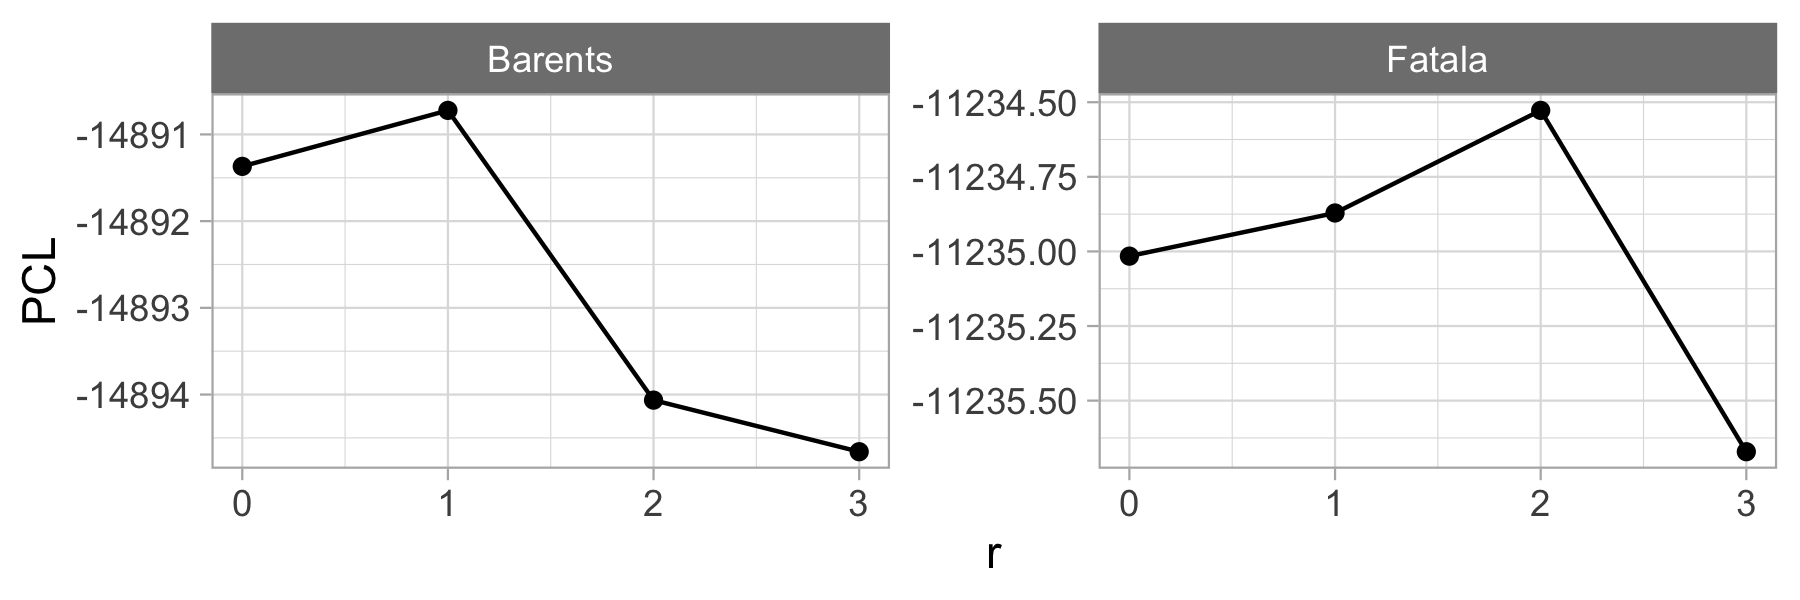
\includegraphics[width=10cm]{figs/selec_model_applis.png}
    \caption{Pairwise composite likelihoods estimates of Barents and Fatala datasets for models including 0 to 3 missing actors.}
    \label{fig:selec}
\end{figure}

% \SR{
% A wider exploration of likely cliques is conducted thanks to a bootstrap approach with $200$ sub-samples. Each of the latter consists of 80\% of the data; sPCA is run on each of them and only the identified clique of the $r$ first principal components are stored, when the studied model involves $r$ missing actors. When $r>1$, the restriction on the clique sizes is lifted. The bootstrap thus yield 200 lists of $r$ initial cliques, from which only unique ones are kept. This approach is more time-consuming, and therefore only used on empirical datasets.
% }{
Regarding the initialization, we performed a wider exploration as compared to the simulation study. To enlarge the list of possible cliques, we applied a resampling version of the procedure described in Section \ref{sec:algoSpec}, and applied it to 200 sub-samples, each consisting in 80\% of the whole data set. This yielded 200 lists of $r$ initial cliques, from which duplicates were removed.
%}

%%%%%%%%%%%%%%%%%%%%%%%%%%%%%%%%%%%%%%%%%%%%%%%%%%%%%%%%%%%%%%%%%%%%%%%%%%%%%%%%
\subsection{Barents Sea}
%data availability ? précisions sur les données, elles viennent d'où

% \SR{30 species of fish were counted in 89 sites of the Barents Sea (shrimp survey in the period April-May 1997, available at  \url{https://www.fbbva.es/microsite/multivariate-statistics/data.html})}{
The dataset was first published by \cite{FNA06} and consists of the abundance of 30 fish species measured in 89 sites in the Barents See in April-May 1997. In addition to abundances, the water temperature was measured in each site. The complete dataset is available at \url{www.fbbva.es/microsite/multivariate-statistics/data.html}. 
Fishes distributions are known to be greatly linked with the temperature. 
Hence to illustrate our methodology, 
% \SR{models were fit\CA{}{ted} without any covariates and with one missing actor, which we denote $h$. $\rm{Cor}(k,temp)$ denotes the absolute Pearson's correlation between $M_k$ (estimated vector of means of node $k$ along all 89 sites) and the temperature.}{
we present the results of the model fitted without any covariate (that is not accounting for the temperature), but including one missing actor (as suggested by Figure \ref{fig:selec}). To assess the ability of the proposed methodology to retrieve the influence of temperature as a missing actor, we report the empirical correlation between the temperature and the conditional expectation of the missing actor $M_h$, which we denote $\corHTemp$.
 
% Runing time
The resampling initialization procedure yielded in 14 different cliques, for each of which a VEM algorithm was run: the mean running time was $6.63$mins with deviation $0.70$ mins. 

% Dependency structure
The edge probabilities involving node $h$ as an endpoint were either very close to 0 or very close to 1, yielding a total of 6 highly probable neighbors of $h$. Figure \ref{fig:barents_adj} shows that many direct interactions are inferred between the corresponding 6 species in absence of a missing actor, which vanish when it is introduced. It also shows that accounting for this actor has only a local effect and that the direct interactions among the other species are preserved, which is consistent with our notion of a missing actor.

\begin{figure}[H]
    \centering
    \includegraphics[width=10cm]{figs/Barents_mat_comp.png} \\\vspace{-2cm}
    \includegraphics[width=10cm]{figs/Barents_net_comp3.png}
    \caption{\textit{Top left:} adjacency matrix of the Barents Sea fishes interaction network for $r=0$  missing actor. The inferred neighbors are gathered in the last 6 columns, so that their interactions are observable in the upper-right corner. \textit{Top right:} adjacency matrix for $r=1$  missing actor. The last column gathers the interactions of the inferred missing actor. \textit{Bottom}: Inferred interaction network with $r=0$ (left) and $r=1$ (right). Colored nodes refer to the inferred neighbors (blue) of the missing actor (yellow). The edges width are proportional to their probability.}
    \label{fig:barents_adj}
\end{figure}

%\begin{figure}[H]
%    \centering
%    \includegraphics[width=10cm]{missing_article/Fig/Barents_net_comp3.png}
%    \caption{Barents Sea fishes interaction network with $r=0$ (left) and $r=1$ (right). Colored nodes refer to the inferred neighbors (blue) of the missing actor (yellow).}
%    \label{fig:barents_net}
%\end{figure}

% Interpretation
In terms of interpretation, Figure \ref{fig:barents_temp} shows that the missing actor is highly correlated with the temperature. It also appears that the abundances of the species neighbor to the missing actor are much more correlated with the temperature (mean correlation = 0.78, sd = .06) than the abundances of the non-neighbor species (mean correlation = 0.46, sd = .27). This example shows the ability of the method to recover an underlying effect that would not be recorded in the data.

\begin{figure}
    \centering
    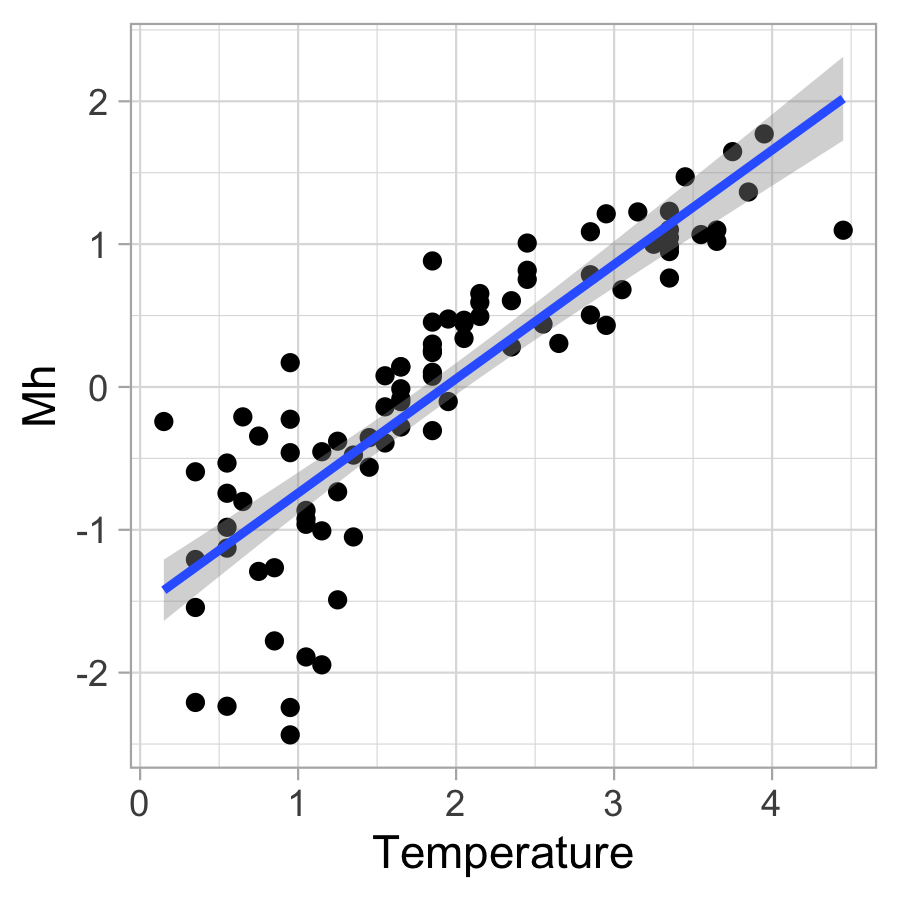
\includegraphics[width=5cm]{figs/Barents_MH_temp_white.png}
    \caption{Missing actor estimated vector of means $M_h$ as a function of the temperature. $\corHTemp=0.85$.}
    \label{fig:barents_temp}
\end{figure}

% \SR{
% Table \ref{tab:barents} then gathers the mean of correlations to the temperature of neighbors and non-neighbors. It appears that neighbors to the missing actor are significantly more correlated to the temperature than other nodes are.
% \begin{table}[ht]
% \centering
% \begin{tabular}{rlrr}
%   \hline
%   $P_{hk}$ & $\corKTemp$  \\ 
%   \hline
%  $<0.5$  & 0.44 (0.25)\\ 
%   $\geq 0.5$ & 0.80 (0.06) \\ 
%   \hline
% \end{tabular}
% \caption{Mean and standard deviation of $\corKTemp$ in relation with node $k$ being inferred as a neighbor ($P_{hk}\geq 0.5$) of missing actor $h$ or not ($P_{hk}< 0.5$).}
% \label{tab:barents}
% \end{table}
% }{
%} 

%\begin{figure}
%    \centering
%    \includegraphics[width=9cm]{missing_article/Fig/Barents_mat_comp.png}
%    \caption{\textit{Left:} adjacency matrix of Barents Sea fishes interaction network for $r=0$. The inferred neighbors are gathered in the last 6 columns, so that their interactions are observable in the upper-right corner. \textit{Right:} adjacency matrix of Barents Sea fishes interaction network for $r=1$. The last column gathers the interactions of the inferred missing actor.}
%    \label{fig:my_label}
%\end{figure}

%\begin{figure}[H]
%    \centering
%    \includegraphics[width=10cm]{missing_article/Fig/Barents_net_comp3.png}
%    \caption{Barents Sea fishes interaction network with $r=0$ (left) and $r=1$ (right). Colored nodes refer to the inferred neighbors (blue) of the missing actor (yellow).}
%    \label{fig:my_label}
%\end{figure}

%%%%%%%%%%%%%%%%%%%%%%%%%%%%%%%%%%%%%%%%%%%%%%%%%%%%%%%%%%%%%%%%%%%%%%%%%%%%%%%%
\subsection{Fatala River}
% \SR{
% The R package \texttt{ade4}  provides with the baran95 dataset which gathers the abundances of 33 species of fish on 90 locations of the Fatala River in Guinea. Data sampled between June 1993 and February 1994, which we organize in dry and rainy seasons; dates and sites are available as dataset categorical covariates.
% %
% Again models are fit with no covariates, and here two missing actors are inferred, which we denote $h1$ and $h2$. As models include more than one missing actor, the best VEM is selected under the constraint $\log sd(M_h)\geq -20$ for $h\in \{h1, h2\}$. This constraint ensures that the corresponding marginal variance of each missing actor is not too high, which would mean that the algorithm did not learn a lot about them. In other words, this ensures the algorithm succeeds in finding the desired number of missing actors. \\
% %
% The bootstrap method gives 60 unique  lists of two possible initial cliques and the mean running time for a convergence with precision $1e-3$ is $11.33$ min with deviation $1.47$; 14 did not reach convergence and the algorithm stopped after 100 iterations. \\
% %
% The best fit gives vectors of means $Mh1$ and $Mh2$ corresponding two each missing actor. Figure \ref{fig:Fatala} shows the plot of $Mh1$ against $Mh2$ colored with either one of the available covariates. It is very interesting to see that $Mh1$ is linked to the Site covariate, as it clearly separates kilometer 3 from kilometer 46 which are the first and last locations. On the other hand $Mh2$ seems linked with the Season covariate, even if the separation is less obvious.
% }{
\cite{baran1995dynamique} collected the abundances of 33 fish species in 90 sites along the Fatala River in Guinea between June 1993 and February 1994. The data are available from the R package \texttt{ade4} on CRAN \citep{dray2007ade4}, along with the date and site of collection, from which we deduce the season (dry or rainy). Again the model was fitted without any covariates, but with two missing actors, as suggested by Figure \ref{fig:selec}. \\
%
The resampling initialization procedure yielded in 60 different cliques, for each of which a VEM algorithm was run: the mean running time was $11.33$ min (sd = $1.47$ mn). 14 VEM did not reach convergence (with tolerance $\varepsilon = 1e-3$) after 100 iterations. We filtered out the results obtained from the different initializations, when the algorithm obviously ended in a degenerate solution ($\Var(M_h) < \exp(-20)$). \\ 
%
% %\SR{
% Figure \ref{fig:Fatala} shows the scatterplot of estimated conditional mean of the two missing actors $(M_{h_1}, M_{h_2})$ in each site, colored with either one of the available covariates (site and season). $M_{h_1}$ is obviously linked to the site and separates most upstream locations (kilometer 3) from most downstream locations (kilometer 46). On the other hand $M_{h_2}$ seems linked with the Season covariate, even if the separation is less obvious. Similarly, the second missing actor shows a clear relation with the season. \\
% % 
% Again, the retrieved missing actor each correspond to an underlying effect that rules fish species abundances. The clear separation between the two effects is reinforced by the assumption the missing actors are independent from each other, which obviously holds for locations ans seasons. \\
% }{
Figure \ref{fig:Fatala} shows the scatterplot of the estimated conditional mean of the two missing actors $(M_{h_1}, M_{h_2})$ in each site, colored with either one of the available covariates (site and season). The missing actor $h_1$ is obviously linked to the site and separates most upstream locations (kilometer 3) from most downstream locations (kilometer 46). This actor has 11 highly probable neighbor species.
% \textcolor{red}{comparer les anova Poisson pour les voisins / pas voisins}
Again, this retrieved missing actor corresponds to an underlying effect (in this case: geography) that rules fish species abundances. \\
% 
The second missing actor seems to be linked with the season but with a less clear separation. Also the variability of $M_{h_2}$ is much smaller than this of $M_{h_1}$. This effect is therefore questionable, which brings us back to model selection. As mentioned above, we used a procedure based on cross-validation, which may  be prone to select too complex model \citep{shao1993linear,friedman2001elements,arlot2010survey}. The definition of a grounded model selection criterion for structure inference in presence of missing actors remains open.
%}

%\textcolor{red}{[C'est un peu dommage de finir comme ça mais bon...]}
 
\begin{figure}[h]
    \centering
    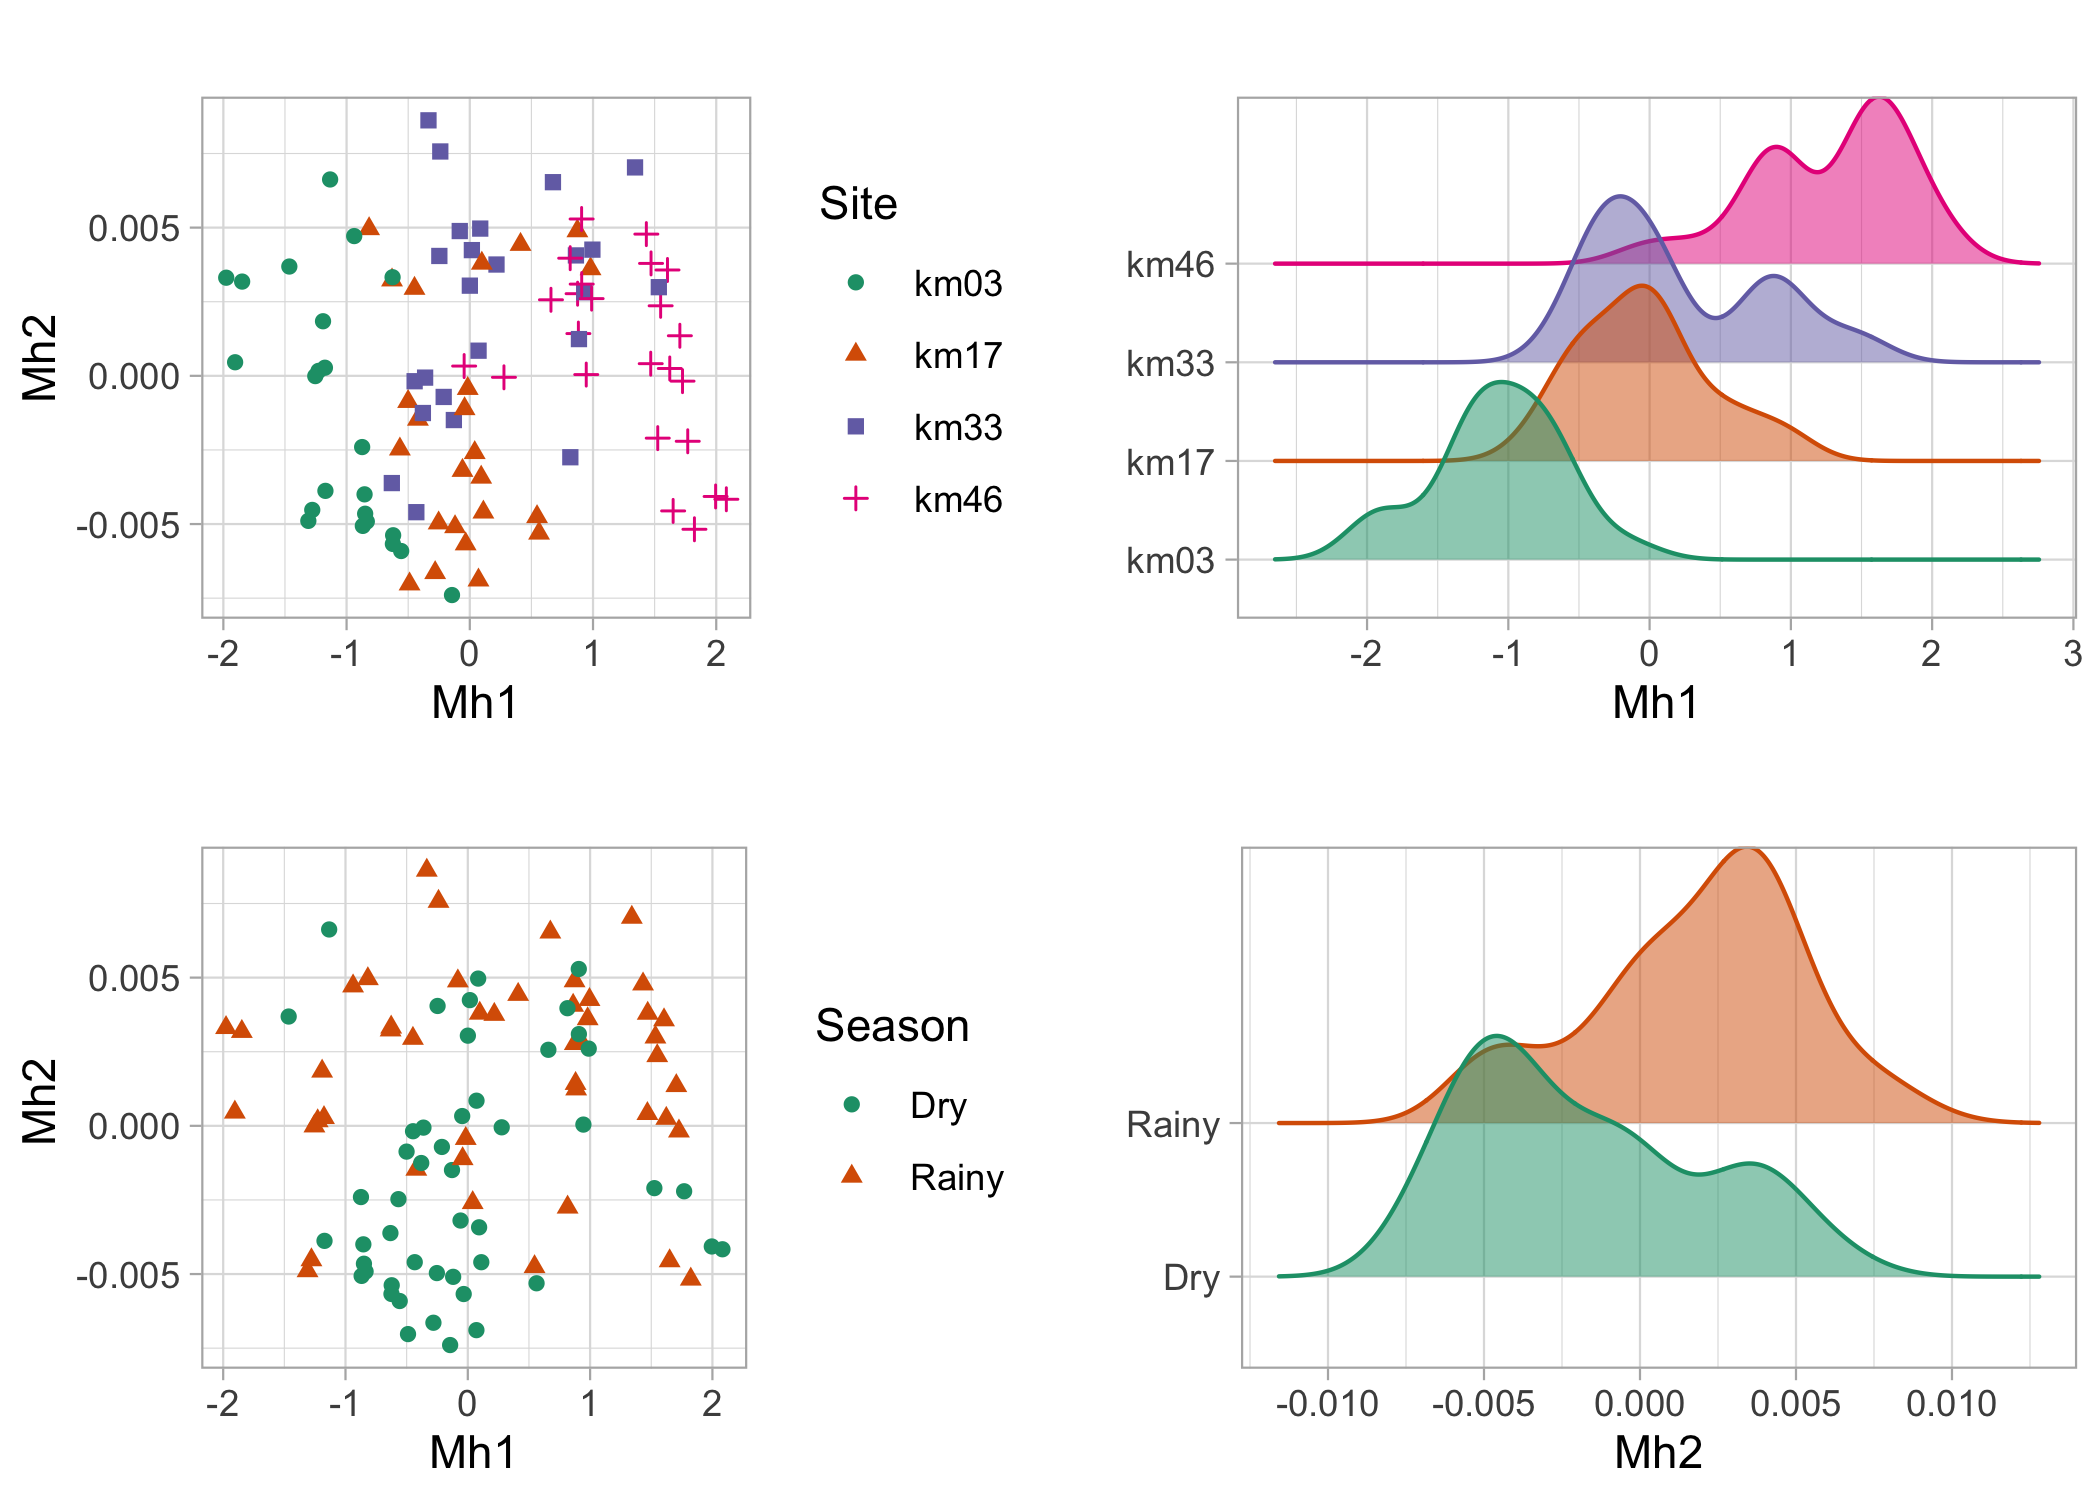
\includegraphics[width=12cm]{figs/Fatala_MH2.png}
    \caption{Estimated means $M_{h_1}$ and $M_{h_2}$ of the two inferred missing actors. Left column: scatterplots $M_{h_1}$ vs $M_{h_2}$ with site (top) and season (bottom) color code. Right: distribution of the estimated means across sites. Top right: distribution of $M_{h_1}$ in each location, bottom right: distribution of $M_{h_2}$ in each season.}
    \label{fig:Fatala}
\end{figure}

